\subsection{Полная проверка и эффекты обозначений}
Все 320 запланированных генераций дали полные программы и результаты штатной проверки: повторных генераций, пропусков и превышений времени оценки нет. Среди 316 исходов с пригодными контролями 173 успешны и 143 неуспешны. Четыре исхода задачи /59 сохранены в полном приложении (три успеха и один провал), но не входят в статистику качества. Таблица~\ref{tab:seg80-groups} содержит итоги четырёх условий.
\begin{table}[t]\centering\small
\caption{Независимое дополнение на 80 задачах. RB/NB: ролевые/нейтральные обозначения с заголовками; RP/NP: те же обозначения в абзаце. V --- средняя стандартная условная API-стоимость наблюдаемого кандидата, а не платёж.}\label{tab:seg80-groups}
\begin{tabular*}{\linewidth}{@{\extracolsep{\fill}}lrrrrr}\toprule
Режим & Получено & Успех/оценено & Успех (\%) & Токены & V (USD)\\
\midrule
RB & 80/80 & 44/79 & 55.70 & 4415 & 0.007244\\
NB & 80/80 & 44/79 & 55.70 & 4431 & 0.007320\\
RP & 80/80 & 42/79 & 53.16 & 4331 & 0.006881\\
NP & 80/80 & 43/79 & 54.43 & 4331 & 0.006884\\
\bottomrule\end{tabular*}\end{table}


При заголовках роли и нейтральные этапы решают по 44 из 79 пригодных задач (55.70\%); парных побед и поражений по три. В сплошном тексте роли решают 42 задачи (53.16\%), нейтральные этапы --- 43 (54.43\%), при пяти победах и шести поражениях. Разности ролей равны соответственно 0.00 процентного пункта, описательный 95\% интервал [-6.33,+6.33], и -1.27 [-10.13,+6.33]. Оба точных двусторонних теста Мак-Немара имеют исходное и скорректированное по Холму $p=1$ (табл.~\ref{tab:seg80-tests}). Широкие интервалы не устанавливают эквивалентность и не исключают содержательно значимый эффект качества.
\begin{table}[t]\centering\small
\caption{Два заранее заданных ролевых контраста. Разности и описательные 95\%-интервалы бутстрэпа по задачам даны в процентных пунктах. W/L --- дискордантные пары; поправка Холма охватывает оба точных двусторонних теста Мак-Немара.}\label{tab:seg80-tests}
\begin{tabular*}{\linewidth}{@{\extracolsep{\fill}}lrrrrr}\toprule
Контраст & Пары & Разность [интервал] & W/L & $p$ & $p_{\rm Holm}$\\
\midrule
RB - NB & 79 & $+0.00\;[-6.33,+6.33]$ & 3/3 & 1.0000 & 1.0000\\
RP - NP & 79 & $-1.27\;[-10.13,+6.33]$ & 5/6 & 1.0000 & 1.0000\\
\bottomrule\end{tabular*}\end{table}


Описательные разности заголовков относительно сплошного текста составляют +2.53 пункта [-5.06,+10.13] при ролях и +1.27 [-6.33,+8.86] при нейтральных обозначениях. Их взаимодействие равно +1.27 [-10.13,+12.66]. Ни сравнения ролей, ни оценки оформления не устанавливают преимущества по качеству. Проверяется наблюдаемая инструкция, а не фактическое возникновение независимых внутренних ролей.

\subsection{Ресурсы и связь с основным экспериментом}
Счётчики доступны для всех 320 вызовов: 932\,812 входных токенов, включая 797\,696 кешированных, и 467\,794 выходных, включая 373\,494 reasoning. Общий расход --- 1\,400\,606 токенов, оценка по стандартным API-тарифам --- USD 2.2662372, чувствительность без кеш-скидки --- USD 2.804682. Это оценка подписочных вызовов, а не платежи за API.

Для ролей относительно нейтральных этапов при заголовках отношение токенов равно 0.9964, отношение стоимости --- 0.9897. Парная средняя разность стоимости составляет USD -0.0000756 с описательным интервалом [-0.0011090,+0.0008682]. В сплошном тексте отношения равны 0.9998 и 0.9996, разность стоимости --- USD -0.0000029 [-0.0011391,+0.0011926]. Без кеш-скидки отношения стоимости составляют 0.9940 и 1.0022; оба интервала ресурсной разности включают ноль. Все четыре контраста представлены на рис.~\ref{fig:seg80-effects}.

\begin{figure}[htbp]\centering
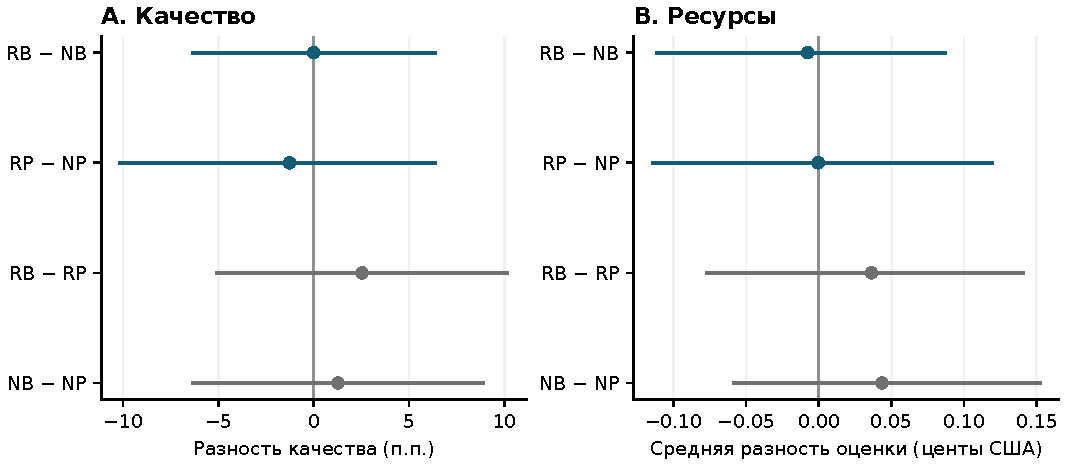
\includegraphics[width=\linewidth]{figures/segregation80/effects_ru.pdf}
\caption{Независимый эксперимент: парные разности качества (процентные пункты) и оценки по API-тарифам (центы США на кандидата), описательные 95\% бутстрэп-интервалы по задачам. Первые два контраста образуют основное семейство тестов качества; контрасты оформления описательные. RB/NB --- ролевые/нейтральные заголовки, RP/NP --- роли/этапы в сплошном тексте.}\label{fig:seg80-effects}
\end{figure}

Таким образом, снижение стоимости одношаговых ролей на 18.45\%, наблюдавшееся в основной серии, не получило убедительного повторения при изменённых формулировках и оформлении. Межсерийное сравнение остаётся описательным, поскольку различаются задачи, инструкции, время исполнения, среда и лимит времени; формальный тест неоднородности не заявляется. Дополнительные оценки ограничивают обобщение ресурсного результата на одни названия ролей, не опровергая основную серию, не доказывая нулевой эффект и не проверяя трёхвызовную топологию. Два проспективных анализа сохраняются раздельно.
